%!TEX root = project.tex

\chapter*{About this project}
\paragraph{Abstract}
A brief description of what the project is, in about two-hundred and fifty words.

\paragraph{Author}
Emmanuel Osabuehien (G00373559)

\chapter{Introduction}

\section{Overview}

In this chapter, I will give a quick overview on my Introduction to my dissertation, where we will be going through some of the research conducted before the development of the application.\\ \\
Here I will be giving you insight into what my project is and why I decided to make this app.\\ \\
We will also be talking about the negatives and positives of most apps in my project field and the benefits of curating such an app.\\ \\
We will lastly be going through the software requirements that I plan to complete by the end of the apps developmental process.

\section {Meal Planning Application}

In this section, I will be giving a brief introduction into what my project is and why I have chosen to do it.\\ \\
My project is known as a Meal Planning System, this is a system that offers meals for people so they can plan and decide whats meet their dietary requirements and budget.

\begin{center}
  \begin{figure}[H]
    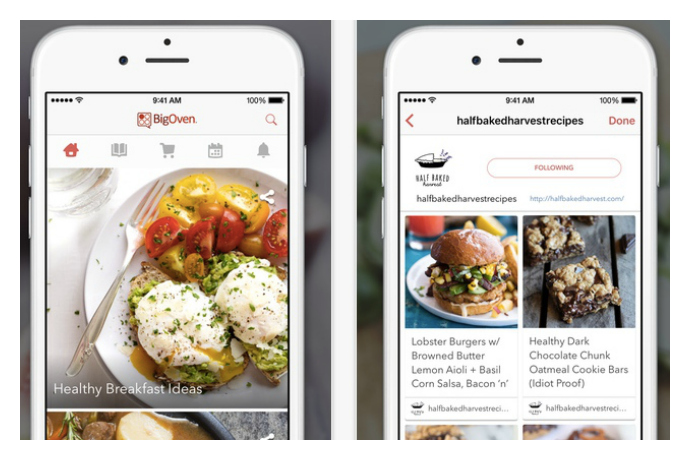
\includegraphics[width=\textwidth]{img/mealplanningpic.jpg}
    \caption{Mean Planning Example}
    \label{fig: Example of a Meal Planning System}
  \end{figure}
\end{center}

\subsection{What is a meal planning application?}

A meal planning application is an app that you plan several weeks of meal plans/grocery lists and then put those weekly meal plans into a rotation, this system is designed for users to eat healthier, giving users the decision to think about what they would like to eat and will those select items provide your body with nourishment.

\subsection{History of meal planning}

First, time devoted to cooking has decreased: in the United States, it has been reduced from 1:63 hour per day in 1965–1966 to 58 min in 2006–2007. Additionally, the source of food consumed has changed: people consume less food prepared at home, whereas foods prepared away from home represent an increasing part of the diet. \\ \\
These studies highlighted that the consumption of food prepared away from home is associated with a lower quality diet and a higher body mass index, whereas benefits have been attributed to home-prepared food. \\ \\
Previous research emphasized that individuals with lower cooking skills were more likely to consume away from home food such as ready meals or take-out meals from fast food or restaurants. \\ \\
To face time pressure, a series of qualitative studies highlighted that parents resort to food choice coping strategies, such as meal simplification, taking out, or meal planning despite their potential impact on diet quality. \\ \\
Among these strategies, time management skills and in particular meal planning, which consists in deciding ahead the foods that will be eaten in the next few days, has been previously suggested as a solution to balance competing time demands and reduce barriers to healthy dietary practices. \\ \\
Studies performed on general populations showed that meal planning was positively associated with frequencies of home food preparation and family meal, as well as the presence of fruits for dinner. \\ \\
In the present study, we hypothesize that meal planning might encourage home meal preparation, and therefore have beneficial effects on dietary quality and consequently on weight status. \\  \\
Then, we investigated the relationships between meal planning and diet quality, based on adherence to nutritional guidelines, energy, macronutrients and food group intakes, as well as food variety.

\subsection{Why am I making meal planning system?}

Q. Why have I choose an meal planning system? \\ \\
A. I believe this is completely correct in scope for my a software project as can conjure up many queries for me as a developer, examples of this may be how can I protect user information and how can I create a functional customer to supplier relationship within this software. This line of questioning is necessary as it is a much needed addition as I gain experience as a developer. I believe that this application is great as a developer as I gain a understanding from both a perspective of both a developer and user and some of the issues both can face. This application will enhance the skills all software developers should have time management, cross-platform software, database knowledge and problem solving. This type of application is needed for a variety of different users, for example myself as a student living away from home, I have now work independently and try provide for myself which is hard due to not always having to fund to go out and buy a vast amount of ingredients, this app can help from young people, people with deficiencies, people planning to lose wight, etc. with these sorts of issues.

\subsection{What are some of my issues with most meal planning systems and how do I think they can be improved?}

Many users of a typical meal planning systems depending on who you ask tend to have many problems with many modern meal planning apps, this can include apps such as 'Paprika' and 'MealBoard'. Some of the problems I will discuss below and give my take on how to combat these issues \\ \\
\textbf{Lack of Information: }Many users of meal planning apps will tell you how their is a lack of information given to a regarding nutrients the body needs.
My plan to combat this is by presenting users with a graph that shows what is the percentage of food types necessary for a person to consume in a day. \\ \\
I will also present users with recipes/meals and proper instructions into how to prepare and cook these meals instead of just giving users a list of meals they would have to research by themselves.
\\ \\
\textbf{Practicality: }I aim to provide an eye-catching user interface by using the react libraries available such as React Bootstrap, ChartJS and React Hook Form to provide users with a simple meal planning app with a navigation bar to move through different pages and providing exciting features.\\ \\
\textbf{Lack of Customization: }I aim to make this app feel personal to the user, it will involving adding graph/charts showing expenditure towards meals giving the user a very different experience than what they are used to.\\ \\
\textbf{Economic Consideration: }Most apps regarding meal planning will not take into consideration users economic struggles, which is something I believe should be always kept in mind, to combat this issue I will provide a list of meals from cheap to expensive to make so users will not be worried about their expenditure when choosing meals. 
\\ \\
\textbf{User Interface: }The user interface on most meal planning apps are not easy on the eye and quite dull. I plan to make one of more quality and vibrant to visualize for a user so they are more intrigued when they view the app. \\ \\
These apps may also be difficult to understand how to move around, I plan to make my app so it will be a quite easy to for a new user to navigate around.

\section {MERN Stack}
In this section, I will be talking about a MERN Stack, we will be going through the points of what it is, why I am using it and how is it employed.
\begin{center}
  \begin{figure}[h!]
    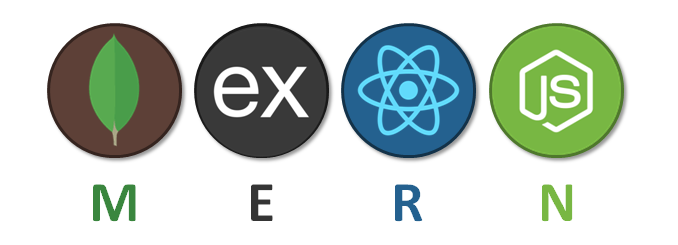
\includegraphics[width=\textwidth]{img/mern-stack.png}
    \caption{MERN Stack Logo}
    \label{fig: MERN Stack Image}
  \end{figure}
\end{center}
Now to put everything into context MERN is an acronym made up of the key technologies that make up the stack itself.
\begin{itemize}
\item M = MongoDB
\item E = ExpressJS
\item R = ReactJS
\item N = NodeJS
\end{itemize}
This is a big reason why I chose to use a MERN Stack for my project as this technology provides a smooth, simple way to make a full-stack web application that can be explained as follows. \\ \\
\textbf{MongoDB} is a open source, cross platform, NoSQL document-oriented database which is used to store a large amount of data in documents and collections. \\ \\
\textbf{ExpressJS} is server-side, back end web application framework that is used for NodeJS needed to write simple and secure applications. \\ \\
\textbf{ReactJS} is a open source, front end JavaScript Library used to create graphical user interfaces of web applications. \\ \\
\textbf{NodeJS} is a open source, cross platform back end JavaScript run time environment, running the JavaScript code outward of the browser. \\ \\

\subsection{MongoDB}

\begin{figure}[H]
  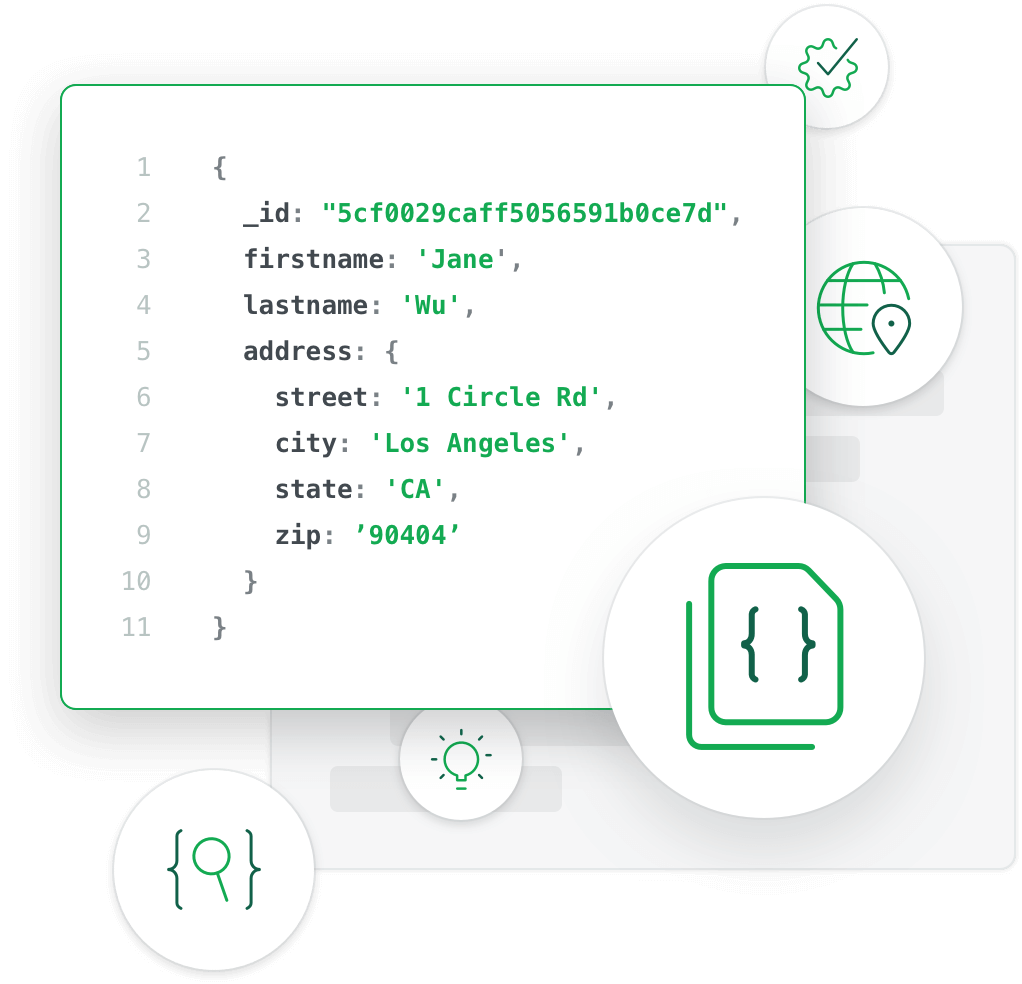
\includegraphics[scale=0.35]{img/mongodbeg.png}
  \centering
  \caption{Example of Mongo Database}
  \label{fig: Mongo Database}
\end{figure}

The reason I decided to use MongoDB as opposed to MySQL or other services available for my database management can be broken down into a couple of reasons, one of the big reasons is it's growth in popularity but removing that key factor MongoDB has many advantages over most services in this area including:

\begin{itemize}
\item\textbf{MongoDB} can handle large volumes of unstructured data
\item\textbf{MongoDB} has the ability to scale up quickly
\item\textbf{MongoDB} allows schemas to be flexibile due to it's data models
\item\textbf{MongoDB} is constantly evolving
\end{itemize}

\subsection{ExpressJS}

\begin{figure}[H]
  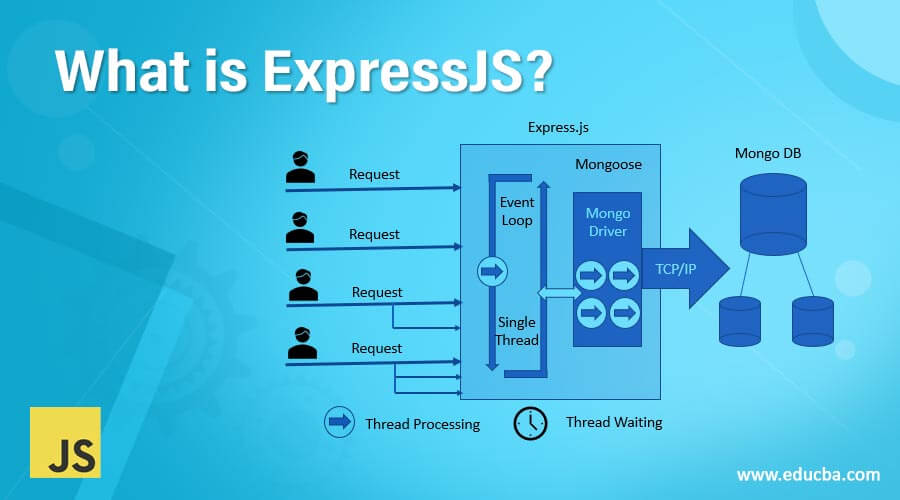
\includegraphics[scale=0.4]{img/whatisexpressjs.jpg}
  \centering
  \caption{Example of an ExpressJS process}
  \label{fig: What is ExpressJS?}
\end{figure}

The reason I chose ExpressJS as opposed to other frameworks for my back end development is due to it's high quality status of performing a server-side connection and it's ability for unfamiliar users to easily use, learn and understand, other positives include:

\begin{itemize}
\item\textbf{ExpressJS} allows users to use the same programming language as the front end
\item\textbf{ExpressJS} has the ability to scale your application quickly
\item\textbf{ExpressJS} can easily connect to databases such as MongoDB or MySQL
\item\textbf{ExpressJS} works well with NodeJS
\end{itemize}

\subsection{ReactJS}

\begin{figure}[H]
  
\includegraphics[scale=1.0]{img/reatcjspic.png}
  \centering
  \caption{Example of React App Symbol}
  \label{fig: React App Symbol}
\end{figure}

The reason I chose ReactJS as it is a JavaScript library that is great for building user interfaces and framework that has been on the rise since it's conception in 2013, ReactJS offers many services and features when creating an easy to navigate user interface, other advantages include:

\begin{itemize}
\item\textbf{ReactJS} is easy to use and understand
\item\textbf{ReactJS} provides reusable components of HTML code
\item\textbf{ReactJS} offers a scope where developer can test and debug code
\end{itemize}

\subsection{NodeJS}

\begin{figure}[H]
  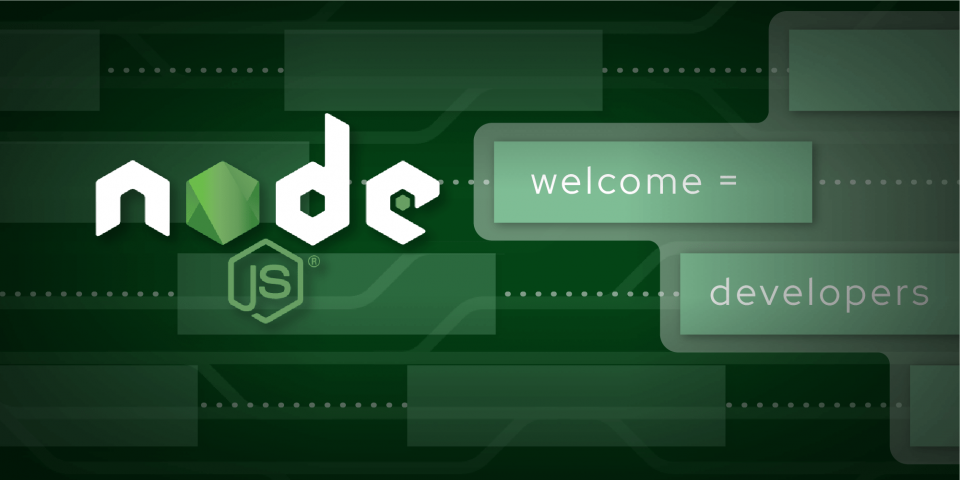
\includegraphics[scale=0.5]{img/nodejspic.png}
  \centering
  \caption{Image of NodeJS Background}
  \label{fig: NodeJS Background}
\end{figure}

The reason I chose NodeJS because it because of server-side security, what it also offers, which includes various tools and libraries useful in web applications and it's ability to easy handle server-side requests, other advantages include:

\begin{itemize}
\item\textbf{NodeJS} has the ability to scale up quickly
\item\textbf{NodeJS} is a very flexible run time environment
\item\textbf{NodeJS} is easy to use, learn and understand
\item\textbf{NodeJS} offers cross-platform development, for example you can connect a mobile app link to a desktop app
\end{itemize}

\section{Positives and Negatives of Meal Planning Systems}

In this section, I will discuss both the positives and negatives of meal planning applications

\subsection{Positives}

\begin{itemize}
\item Aiming for weight loss goals
\item Easy to prepare for shopping
\item Allows for better money management
\item Saves users time and energy
\item System offers users a wide variety of ideas to use
\item It might be able to offer some nutritional knowledge
\end{itemize}

\subsection{Negatives}

\begin{itemize}
\item Recipes may not be up to user satisfaction
\item It means setting a schedule and plan and sticking as close to it as possible
\item It takes planning and discipline to meal plan, that you might not have
\item Inflexible and don’t account for varying needs of the body
\end{itemize}

\section{The Benefits of Meal Planning Systems}

In this section, I will discuss the benefits of a meal planning application

\subsection{Health Goals}

 Cooking meals at home increases your chance of reaching health goals, whether or not they are planned to lose weight, improve heart health or keep blood sugar steady, meal planning is what gives you ingredients and resources to actually make this happen on a daily basis.

\subsection{Budgeting}

Meal planning makes it easier to cook more at home, and shoppers can save even more by weekly sales into planning. So the next time you're budgeting for an expense, consider meal planning to help save you money on a set basis.

\subsection{Enables Variety and Gives Control}

Meal planning is often associated with increased food variety, which is key to  a healthy diet that increases your goal of meeting nutritional needs.

Meal Planning also gives you control and choice over ingredients as it is easier to avoid food allergens and to incorporate ingredients that support diets for specific health problems

\subsection{Streamlines Shopping and Decreases Food Waste}

Meal planning allows users to set out their list of ingredients to obtain based around their meal plan, reducing the time and money spent to constant shopping trips.

You are also most likely to make use of forgotten food items that are just stored away, reducing the amount of food waste and unneeded shopping trips by utilizing what you already have on hand.

\subsection{Decision Fatigue}

Meal Planning helps to alleviate the stress and fatigue when deciding what to meals you need to make throughout the day as users can stock up ingredients and have multiple planned meals where they have a wide variety of options to choose from.

\section{Software Requirements}

In this section, I will give a list of the software requirements I intend my project to achieve

\begin{itemize}
\item\textbf{Login: }If user has an account, they are required to login to use application
\item\textbf{Register: }If users don't have an account, they are required to register an account and login to use application
\item\textbf{Logout: }Users can logout if application is not in use
\item\textbf{Forget Password: }If users can't access account/forgot their password, they can retrieve their account by following process provided
\item\textbf{Add Meal: }Uses can add meal into the listing page
\item\textbf{List All Meals: }Users can access listing page where they can view all meals that have been added
\item\textbf{Fetch Meal: }Users can retrieve the meal that they have added to the listing page
\item\textbf{Delete Meal: }Users can delete the meal that they have added to the listing page
\item\textbf{Edit Meal: }Users can update the meal that they have added to the listing page
\item\textbf{Cookies: }The application must use cookies to memorize information during visits and maintain sessions.
time-frame max of a day.
\item\textbf{Security: }Users login details must be encrypted and secure so they cannot be accessed by another user
\end{itemize}

\chapter{Context}

\section{Overview}

In this chapter, I will give a a more clear context on the contents of this document.\\ \\
We will go through the objectives that have been laid out and to be completed during the duration of development.\\ \\
I will briefly discuss each chapter in the document and the contents that each chapter contains.\\ \\
Finally, I will talk about how the project is structured in my GitHub repository including the files for this very document as well as the source files for the application. 

\section {Objectives}

In this section, I will discuss the key objectives that I intend to carry out for this web application. \\ \\
The objectives include:

\begin{itemize}
\item To create a multi-user, functioning web application that can be accessed
\item To an attractive, simple and easy to understand graphical user interface that users can operate without difficulty
\item To provide a system where users can plan out their meals
\item To provide users a system keep track of dietary goals
\item To provide users with nutritional education
\item To provide a multi-user app with a secure database of users where login details are encrypted
\item To provide a REST API to my service to allow users to perform requests
\end{itemize}

\section {Chapters}

In this section, I will give a brief overview of what each chapter in my dissertation contains.

\subsection{Introduction}

In this chapter, this is just an introduction of the project, where we what is the project, why I choose to make this project and use the technology I utilized, provides what are the key objectives of this project and give the viewer an idea on what this dissertation contains.

\subsection{Context}

As is evident by the title of this chapter, in this chapter I will discuss the context of my project, the importance and rise of web-based issue ticketing systems, the benefits and drawbacks of meal planning apps and how convenient they came to be in modern computer science especially in a software project collaborative setting.

\subsection{Methodology}

In this chapter, I will discuss my approach to this project, the methodology and testing I used for this project and why I chose a certain type of methodology and testing, how this had an effect on my project and go into more detail on how the developmental process of my project

\subsection{Technology Review}

In this chapter, I will discuss more about the technical features of the project, all the technologies used in my project at a more conceptual level, how did they affect the developmental process, why did I choose this technology to implement and should a good indication of the research that was undertaken during the creation of the project.

\subsection{System Design}

In this chapter, I will give a detailed explanation of the system architecture i.e., Front End, Back End, Database. There will be an overview of the different components of the system and how they function together when deployed and diagrams to explain and visualize the design of the system.

\subsection{System Evaluation}

In this chapter, I will give an evaluation of my project against the objectives I set out for myself and I will test whether the project meets the user requirements and quality standard. This chapter will include testing of the stability and behaviour of the software and provide graphs/table of the results.

\subsection{Conclusion}

In this chapter, I will summarise various points of the project, I will outline the context, the set objectives and if this was satisfactory to the goals i set for myself. I will discuss the research conducted and highlight the findings I discovered through that process. I will also finally give a list of outcome of the project.

\section {Project Structure}

In this section, I will give a brief overview of the structure of my GitHub repository for viewers.
\begin{figure}[H]
  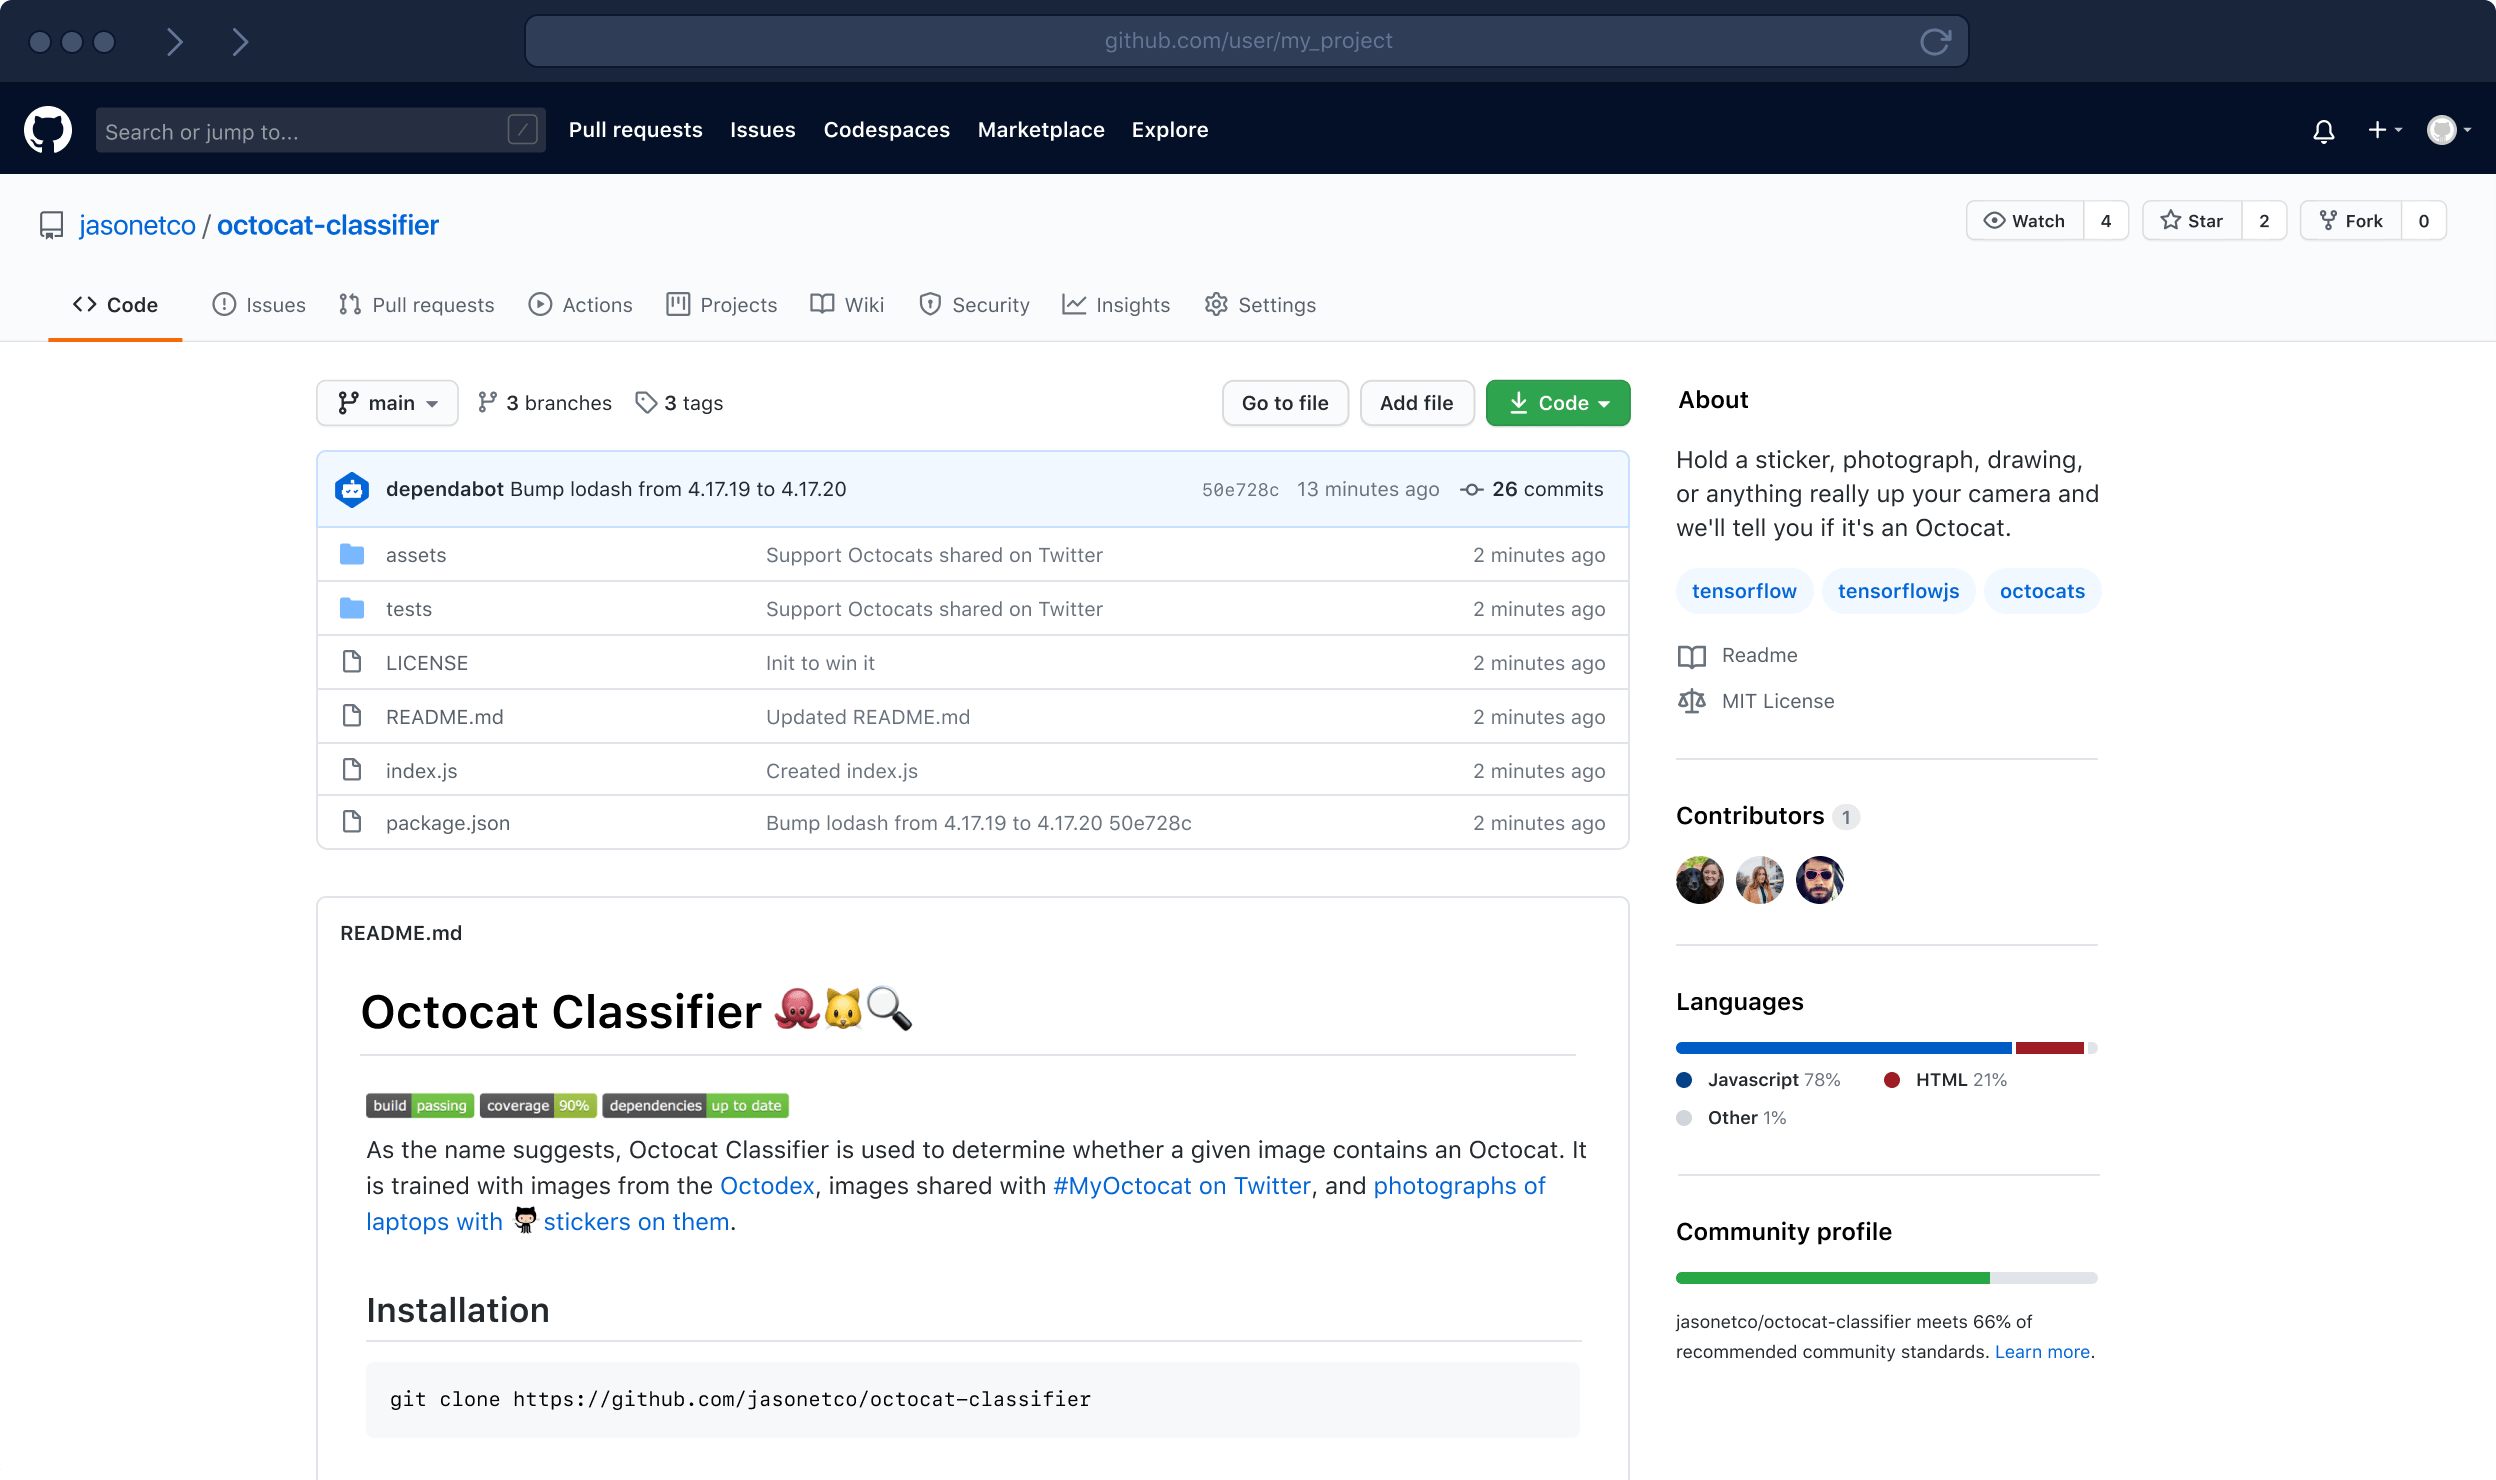
\includegraphics[scale=0.15]{img/githubpic.png}
  \centering
  \caption{Example of GitHub Repository}
  \label{fig: GitHub Repo Example}
\end{figure}
The GitHub repository where this project is located in contains two specific folder, my 'meal-planning' folder which contains the main application of the project (including the front end and back end of my application) and the 'img' folder which contains images used in my application. \\ \\
Apart from this folder my project also contains the files for the dissertation including the 'content.tex', 'project.tex', 'bibliography.bib', the project.tex which contains the cover sheet of the dissertation, content.tex which contains the chapters and sections written and the bibliography.bib which contains the primary, secondary and tertiary resources that are cited in the dissertation. \\ \\ 
There is a README.md file which contains information on why this repository exists, what is in it and how to run the project.  \\  \\
There is also a LICENSE.txt file which is used as a software license agreement. \\ \\
You can view the github by clicking the link as follows: \\  \\ \url{https://github.com/Emmanuel-Osabuehien/AppliedProjectMinorDissertation}

\chapter{Methodology}

\section{Overview}

In this chapter, I will give a quick overview on what is Methodology.\\ \\
During the process of creation my application, I research different approaches, testing and validation to keep my project organized. I adopted the Agile (incremental and iterative) approach for my project, I set up sprints where I set up tasks needed to be completed in a two week period. I also used Test Driven Development (Selenium and JUnit) where I wrote tests with enough code to allow it to pass without bugs, error and fault which I will later on edit this very same code.

\section{Agile Methodology}

In this section, I will discuss what is methodology, different types of methodology and how I implemented methodology in my project.

\subsection{What is Agile Methodology}

Agile is both an incremental and iterative approach to project management and software development that helps teams deliver value to their customers faster according to 'Atlassin', one of the leading examples of Agile framework. Scrum, DevOps, Trello and Jira are only a few examples. The Agile Manifesto outlines the principles that all Agile techniques follow. I'll be utilizing Trello for the duration of this project. Continuous improvement and incremental delivery are key to all Agile approaches.

\begin{figure}[H]
  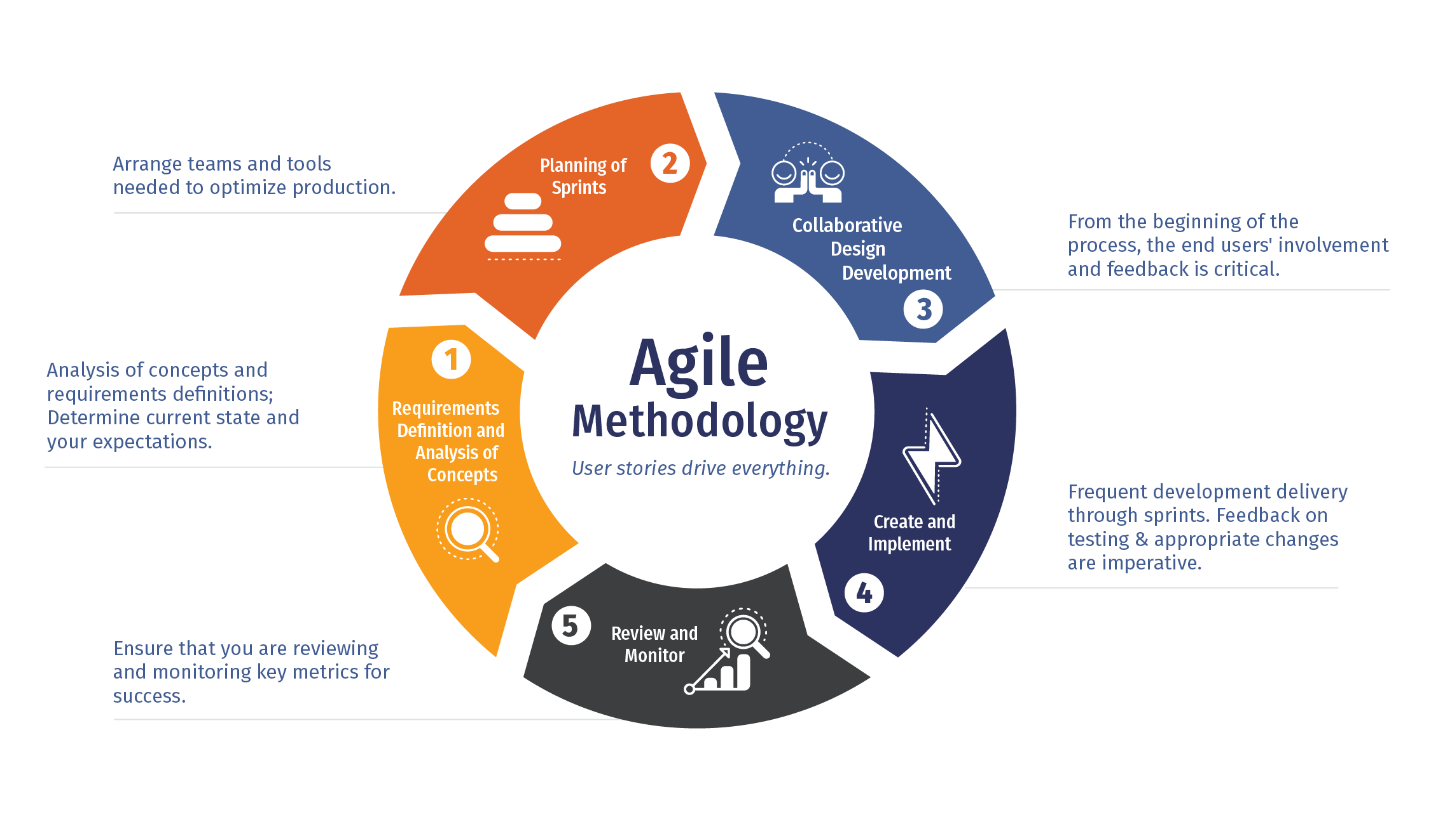
\includegraphics[width=\textwidth]{img/agilemeth.png}
  \caption{Agile Methodology}
  \label{fig: Agile Lifecycle}
\end{figure}

\subsection{Atlassian}

Q. Why did I choose Atlassian as my Agile framework?\\ \\
\begin{wrapfigure}{r}{0.5\textwidth}
  \begin{center}
    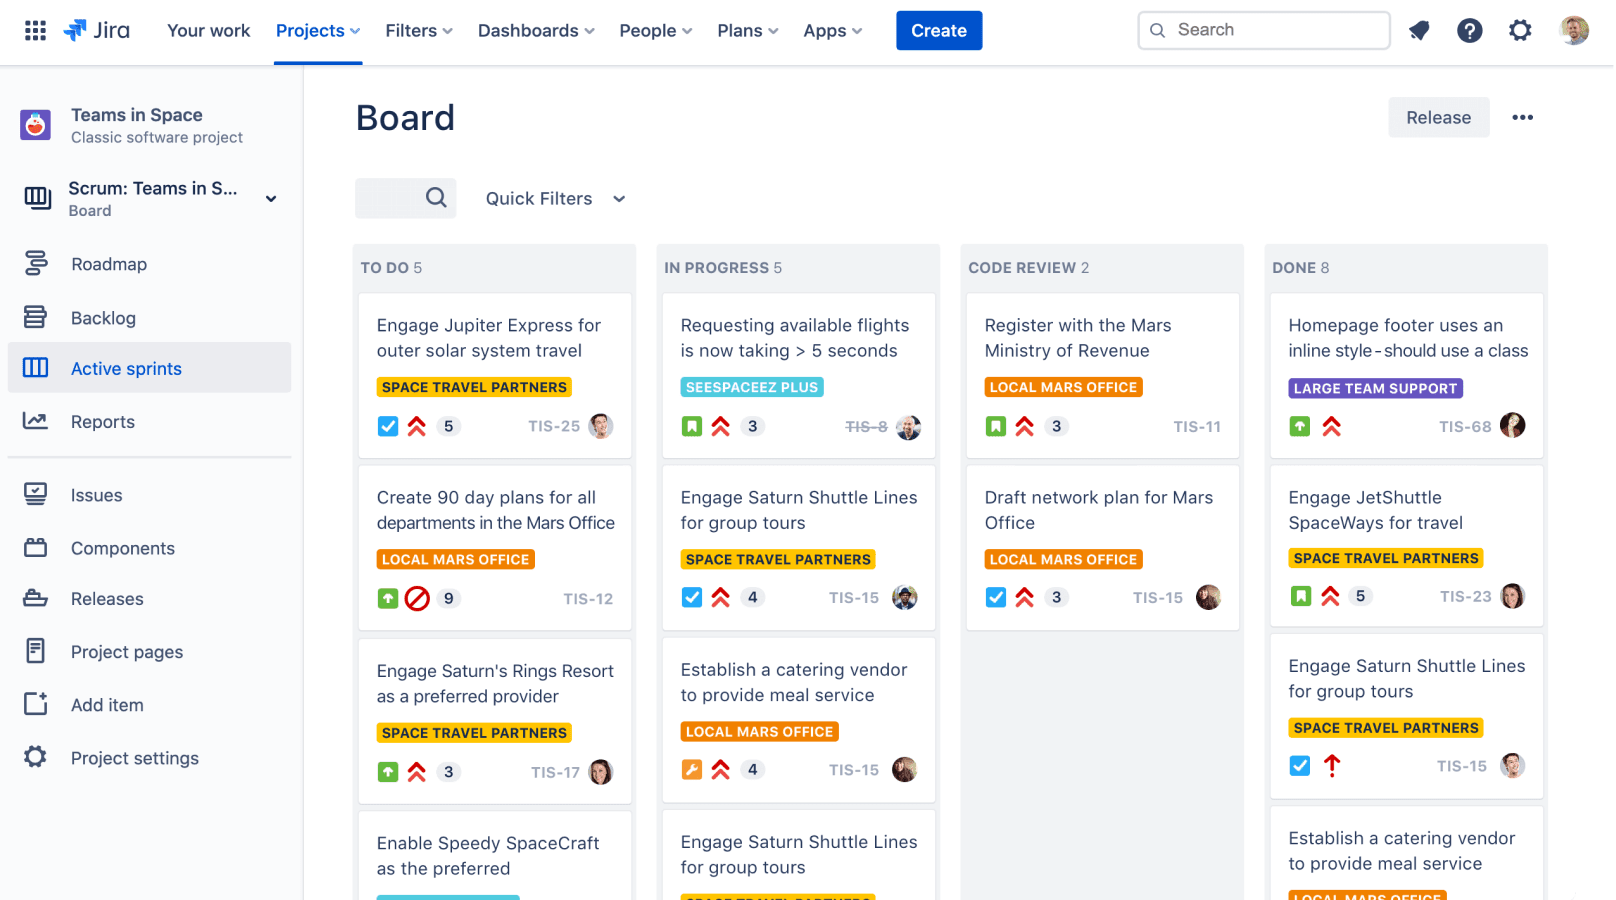
\includegraphics[width=0.75\textwidth]{img/atlasboard.png}
  \end{center}
  \caption{Atlassian Board}
  \label{fig:Example of Atlassian board}
\end{wrapfigure}
A. Atlassian gives the user (or a team) a clear view into the status, progress, and success of projects.  Also, they issue Power Ups to help you work across boards, with an visually appealing user interface.\\ \\
Atlassian also offers features such as:

\begin{itemize}
\item Following production workflow
\item Organizing future projects
\item Keeping track of project developmental process
\item Managing development schedule
\end{itemize}

\subsection{Implementation}

I implemented Trello with my project by connecting my GitHub repository to my project and I set up my sprints in my backlog and added tasks that were to be completed to my working board. I created 3 sections to my board for my working project known as "To Do", "Doing" and "Done", 'To Do' contained issues that were just added, 'Doing' contained issues that are in progress of being completed and 'Done' contained issues that were completed. This helps with the output, outcome and productivity of my project as I can visualize what I need to do and work on in a set schedule. I also have 2 other sections "Backlog" and "Issues", "Backlog" contains all functionality desired in the product and "Issues" contains any bugs, errors or fault in code that needs to be checked.

\section{Validation and Testing}

In this section, I will discuss validation and testing, what they are in terms of software development, different types of software that supply validation and testing and how I implemented testing in my project.

\subsection{Test Driven Development}

Test Driven Development (TDD) is software development approach in which test cases for each functionality are created and tested first and if the test fails then the new code is written in order to pass the test and making code simple and bug-free.

\subsection{Implementation}

I designed and wrote test cases whenever I developed a code to perform a specific functions for my application such as a 'Add a meal to your list' or 'Delete a meal that you have added to the list', after this test was performed I wrote a significant amount of code so the test should not fail and pass and continued to edit the code.

\subsection{End To End Testing}

End To End Testing is a type of software testing to that includes testing a product to check the behaviour of the product runs as intended. This type of methodology is used to recreate real user scenarios to test and validate the product basically aims to replicate real user scenarios so that the system can be validated for code merging and ethics.\\ \\
End To End Testing revolves around testing the application from start to finish during the software development life cycle and is completed running automated testing and manual testing tactics.\\ \\
This testing is applied to make sure that throughout the development of the product to ensure as the product evolves the behaviour of each sub-system works as expected.

\subsection{Unit.js}

Unit.js is just one of the testing frameworks I used to perform automated tests. Unit.js is a open-source framework, it is used to write and run repeatable automated tests. Unit.js is used to perform Java tests and is one of the leading examples of regression testing. This allowed me test the database functions to make sure when the code is run it works smoothly and also make sure certain outputs were correct such as 'Tallying the shopping list cost'.

\begin{figure}[H]
  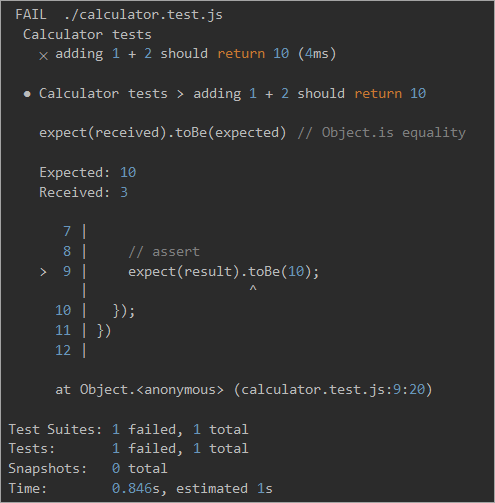
\includegraphics[width=0.77\textwidth]{img/unitjs.png}
  \centering
  \caption{Example of Unit.js Test Case}
  \label{fig: Unit.js Test Case}
\end{figure}

\subsection{Selenium}

I also used Selenium to perform automated tests for my application. 
Selenium is a open-source automated testing framework used to validate web applications across different browsers and platforms that can be used for multiple programming languages such as Java, JavaScript, Python, etc. 
Selenium is used to perform automation testing on such user interfaces and web pages, I implemented Selenium in my React application using Node and this allowed to test the database functions to make sure when the code is run it works smoothly.

\begin{figure}[H]
 \begin{center}
  
\includegraphics[scale=0.25]{img/seleniumlogo.png}
  \end{center}
  \caption{Selenium Logo}
  \label{fig: Image of Selenium Logo}
\end{figure}

\section{GitHub}

In this section, I will discuss the importance of GitHub during the development of my project. \\ \\
GitHub and Git were both very important in the development of my project. I used GitHub to manage all my files and folders regarding my project, repeatedly pushing these files/folders to GitHub whenever progress was made. I used GitHub with my Trello Boards where I would manage issues that arose during the development stages.\\ \\
\begin{wrapfigure}{r}{0.5\textwidth}
  \begin{center}
    
\includegraphics[width=0.35\textwidth]{img/githublogo.png}
  \end{center}
  \caption{GitHub Logo}
  \label{fig:Image of GitHub Logo}
\end{wrapfigure}
GitHub also allowed to me to use multiple branches where I created separate branches 'Main' and 'Master' where I would use Main for my finished code that had been tested and 'Master' for tested certain features which allowed me freedom to perform automated tests for debugging my application. \\ \\
GitHub also provides me with the option of return to previous iterations of my project, so in the case of an errors in the system I can just start again from a previous working and tested version as well as a page dedicated to issues where I can post issues that would then be divided into 2 week sprints.

\section{Issues Faced}

In this section, I will discuss the issues that I faced during the development of my project.

\subsection{Project Timeline}

The project timeline (or organization) was one of the issues I faced during the development of my project as dealing with a variety of different projects and trying to balance them all together was a difficult task that I had to solve. I solved this issue by creating a weekly schedule where I would allocate a select amount of time for different modules and project that I was working on so I didn't focus and stress about one project more than another.

\subsection{Underestimating The Scope}

The project scope was another issue I faced as I went through several ideas for my project and struggled with identifying if any of those ideas was the correct scope for my project. I overcame this obstacle by having weekly meetings with my supervisor where we would discuss on if the scope of my idea was right until coming to a conclusion.

\subsection{Feature Overload}

Feature overload was another issue that was faced during the development of my project as trying to select the right software/technology was difficult as I stressed how multiple types of software would gel together until I decided to use a MERN Stack that all flowed together smoothly and worked well together.

\chapter{Technology Review}

\section{Overview}

In this chapter, I will give a quick overview on different React/JavaScript libraries and frameworks, programming languages, programming software, and REST/Database Architecture that I used to develop my application.\\ \\
During the process of creation my application, I set up a list of features, components and functions that I wanted my application to fulfill by the time of completion. I would at times add to the list during the developmental process of my application. To complete this list, I would research the coding features, frameworks and libraries that would allow me to complete each task I set out for myself and attach each feature, framework or library to a task.

\section{MERN Stack}

In this section, I will discuss the technologies MongoDB, ExpressJS, ReactJS and NodeJS.\\ \\

\subsection{MongoDB}

MongoDB is a cross-platform, document-oriented NoSQL database that uses collections and JSON type documents allowing databases to store high volume data storage, an alternative to most traditional relational databases such as MySQL that use table and rows. The addition of JSON allows data stored to be retrieved and updated. An example of retrieving data can be as follows, here is an example of document that can be modeled in MongoDB:
\begin{minted}{json}
{
  "user": {
    "email": "user1@example.com",
    "password": "password1"
  }
}
\end{minted}
If I can then run code to retrieve specific data that is stored, for example I can retrieve the above user's email as follows:
\begin{minted}{js}
user.email();
\end{minted}
Then once the code is run I should retrieve the user's email as follows:
\begin{minted}{json}
"email": "user1@example.com"
\end{minted}
MongoDB provides key feature such as scalability as you can run hundreds of nodes and millions of documents, replication providing many replica sets that can be used as a primary and secondary set at any time, indexing which improves the  the performance of searches in the database and MongoDB can be run across multiple servers. MongoDB is used by applications such as Uber, Forbes and Lyft.
\subsection{ExpressJS}

ExpressJS is an open-source, server-side web application framework utilized in building and designing either single-page, multi-page or hybrid web applications. There is many advantages to ExpressJS such as it works at a fast work rate, it is easy to learn, it provides predetermined code for developers to use and only knowledge of JavaScript and HTML is necessary. ExpressJS allowed me to utilize it's use of routers to add, edit and delete data to and from our database. \\ \\
Since I decided to use NodeJS instead of Yern, it only made sense to use ExpressJS due to how well they work together. ExpressJS provides middleware that is responsible for making decisions to give the correct responses for the requests made by the client. Express allows us to get and push data in a JSON format which will then have later use and he use of the routers helped me with four key features that I implemented in my app, these features were registration, logging in, adding/deleting meals from list and designing personal shopping lists. \\ \\
A quick example using ExpressJS to set up a simple request handler can be viewed below:
\begin{minted}{JavaScript}
'use strict'

var express = require('../../');

var app = module.exports = express()

app.get('/', function(req, res){
  res.send('Hello World');
});

/* istanbul ignore next */
if (!module.parent) {
  app.listen(3000);
  console.log('Express started on port 3000');
}
\end{minted}

ExpressJS was great in setting up the back end of my application as it allowed me to perform functionality such as adding data, updating data and removing data in our app.

\subsection{ReactJS}

ReactJS is an open-source, client-side JavaScript library used to build user interfaces especially for single-page applications as well as using reusable UI components (many of these components I will discuss in more detail). React was very useful as I was building a large scale web application where data was to be changed quite frequently especially without attempting to refresh the page, for example If I add a meal to my list it should be viewed instantly in the page or whenever a user has logged in our logged out they do so without the page reloading. React also provides many libraries which I will discuss later on that were very useful in creating my application such as Bcrypt which I used to encrypt any user password that was passed to the database. The addition of these libraries as well as my knwoledge of JavaScript and it's relationship with NodeJS and ExpressJS is why I chose ReactJS over software such as Angular which was highly considered.\\ \\
React provides many features such as JSX , UI Components:
 \begin{itemize}
  \item JSX - This is a JavaScript syntax extension.
  \item UI Components - This is necessary when mainting code for large scale projects.
  \item Flux - This helps keeping your data unidirectional.
\end{itemize}
A quick example of employing ReactJS can be seen below:

\begin{minted}{JavaScript}
ReactDOM.render(
<h1>Hello, world!</h1>,
document.getElementById('root')
);
\end{minted}

ReactJS provides many advantages for example, React can be used for both the front end and back end of you application, React uses DOM (Document Object Model) which improves apps performance and the use of components maintaining code improving large scale applications. ReactJS is used by applications such WhatsApp, Netflix and Atlassian.

\subsection{NodeJS}

NodeJS is an open-source, cross-platform, server-side run time environment. Node.js is asynchronous, event-driven enviornment designed to build scalable web applications. NodeJS is integral in handling multiple HTTP requests concurrently these request can be either a GET request, POST request. PUT request and DELETE request. NodeJS was very important in my application as it was needed to perform tasks such as adding users to our database and also adding meals and ingredients to each users documents.\\ \\
The NodeJS website (https://nodejs.org/) provides an example of setting up your run time environment, here if the enviornment is set up correctly, when the user enters https://localhost:3000/ into their browser the message "Server running at https://localhost:3000/ " will be printed in your console and the status code 200:
\begin{minted}{JavaScript}
const http = require('http');

const hostname = '127.0.0.1';
const port = 3000;

const server = http.createServer((req, res) => {
  res.statusCode = 200;
  res.setHeader('Content-Type', 'text/plain');
  res.end('Hello World');
});

server.listen(port, hostname, () => {
  console.log(`Server running at http://${hostname}:${port}/`);
});
\end{minted}
NodeJS contains many advantages such as the speed and performance, providing reusable code, it's ability to handle multiple requests and it's scalability.
NodeJS is used by applications such eBay, Linkedln and Yahoo.

\section{Languages}

In this section, I will discuss the programming languages I used to develop my project.

\subsection{JavaScript}

JavaScript is a high-level, text-based programming language that can be used for both the client and server side. JavaScript allows user to fully engage and interact with web pages as you can use it to calculate, manipulate and validate data and is typically assisted by HTML and CSS.\\ \\
JavaScript is was very useful for my app as JavaScript itself is highly influential in building web apps and web servers as well as developing the interactive behaviors of my web app such as retrieving the users meals data and checking the login details of a pre-existing user.\\ \\
An example of using JavaScript to calculate data can be shown below, where we see an example of a user entering two input values that will be added together:
\begin{minted}{JavaScript}
const num1 = 5;
const num2 = 3;

// add two numbers
const sum = num1 + num2;

// display the sum
console.log('The sum of ' + num1 + ' and ' + num2 + ' is: ' + sum);
\end{minted}

\subsection{HTML}

Hyper Text Markup Language also known as HTML, is a standard markup language used to create, design and structure web pages and also consists of a series of elements, it is typically assisted with the programming languages JavaScript and CSS.\\ \\
A quick example of a HTML document is shown below:

\begin{minted}{HTML}
<!DOCTYPE html>
<html>
<head>
<title>Page Title</title>
</head>
<body>

<h1>My First Heading</h1>
<p>My first paragraph.</p>

</body>
</html>
\end{minted}

\subsection{CSS}

Cascading Style Sheets also known as CSS is a style sheet language that controls the layout of web pages and it is used to describe how HTML elements are to be displayed on screen.\\ \\
Here is an example of code from my meal planning app that I used to design the body of one of the pages:

\begin{minted}{CSS}
body {
    padding: 0px;
    margin: 0px;
    background: #F4F1F1;
    font-family: 'Open Sans', sans-serif;
    color:black;
    font-size: 15px;
}
\end{minted}

\section{JavaScript Frameworks}

In this section, I will go through the frameworks provided by JavaScript that I used to develop my project.

\subsection{Axios}

Axios is a promise-based HTTP Client for node.js and the browser. Axios is what I used to send requests and retrieve responses using the client-server model. Axios played a huge role in my application as it was very necessary in completing the functionality of reading, adding, editing and deleting from my database. I considered using the fetch method instead of using Axios but after deliberating  and researching differences between the two, Axios has the advantage of being better at error handling.

\subsection{CORS}

Cross-Origin Resource Sharing also known as CORS, is a mechanism that allows or prevents requested resources on a server depending on where the request was initiated. I used CORS in my app to load in the API and all the data involved in the API that I used for my project (TheMealDB API), it was an easy decision to choose to use CORS as it was a JavaScript library that I found easy to understand and use.

\subsection{Nodemon}

Nodemon is a command-line interface utility that develops node.js based applications by watching the file system and automatically restarting the node application when a file change has occurred and is detected. I found Nodemon great to use instead of many alternatives due to Nodemon not requiring any additional changes to your code or method of development. Nodemon was simply used as a way to not have to continuously restart my application to make the added changes to my app instead Nodemon will just rerun the app and make the added changes as intended.

\section{JavaScript Libraries}

In this section, I will go through the libraries provided by JavaScript that I used to develop my project.

\subsection{Bcrypt}

Bcrypt is a password-hashing function used to convert a string of input data to a fixed, unpredictable output. I used Bcrypt to encrypt the password of all registered users to enhance user security, so when a user registers into the system with an email and password, the password will be automatically encrypted.

\subsection{Bootstrap}

Bootstrap is a free, open-source toolkit used to create web pages and applications on the applications front end using HTML, CSS and JavaScript templates such as forms, buttons, jumbotrons, etc. I used Bootstrap to design the majority of the web pages for my application using the aforementioned templates that come with Bootstrap.

\subsection{Chart.js}

Chart.js is an open-source, JavaScript library that is used for visualizing data, that allows designers and developers to draw all kinds of charts using the HTML5 canvas element.\\ \\
This includes 8 different charts:

\begin{itemize}
    \item Line Chart
    \item Pie/Doughnut Chart
    \item Bubble Chart
    \item Bar Chart
    \item Radar Chart
    \item Polar Chart
    \item Area Chart
    \item Scatter Chart
\end{itemize}

I used Chart.js to develop a web page that contains a table full of charts that contain different diets that users can follow and read about as each chart contains a hyperlink to a web page giving more insight about a specific diet.

\subsection{JsonWebToken}

JsonWebToken is an open standard used to share security information between the client and a server. I used JsonWebToken to generate Tokens that users can use to log in to their accounts for increased security as opposed to just entering email and password.

\subsection{Mongoose}

Mongoose is a JavaScript library that creates a connection between MongoDB and the Express web application framework. As previously mentioned, I used Mongoose as my way to connect my database to my web application.

\section{React Component Libraries}

In this section, I will go through the libraries provided by React that I used to develop my project.\\ \\

\subsection{Create-React-App}

Create-React-App is a comfortable environment for learning React, in my opinion it is the easiest way to start building a new single-page or multi-page application in React. Create-React-App will automatically set up the coding environment to use JavaScript features. I used Create-React-App to set up my enviorment for my application. 

\subsection{React-Bootstrap}

React-Bootstrap is a front end, component-based library that provides native Bootstrap components as pure React components such as buttons, modals, cards, etc. I used React-Bootstrap as it converts JavaScript to React aimlessly.

\subsection{React-Router}

React-Router is a standard library for routing in React. It enables the navigation of various components in a React Application, allows redirecting the URL of the browser, and keeps the user interface in sync with the URL. I used React-Router to develop and define my routes for my application and connect it to my navigation bar that I implemented into my app.

\subsection{React-Router-Dom}

React-Router-Dom is an node.js package that enables you to implement dynamic routing in a web app. It allows you to display pages and allow users to navigate them. It is a fully-featured client and server-side routing library for React. Look at the above section about 'React-Router' to view why I decided to use React-Router-Dom as the reason is exactly similar to the aforementioned section.

\section{Architectural Styles and Patterns}

In this section, I will discuss the architectural styles or patterns, going through what they are, why they are necessary and the principles to be followed.

\subsection{REST}

Representational State Transfer also known as REST is an architectural style or pattern used to obtain a standard between operating systems allowing communication to be improved upon.\\ \\
Not unlike many other architectural styles, REST has a list of guiding principles that need to be pleased and obtained.\\ \\
These non-negotiable guideline principles are as follow:

\begin{itemize}
    \item \textbf{Uniform Interface:} This is a key constraint which defines the interface between clients and servers. It simplifies and decouples the architecture, which enables each part to evolve independently. The following four constraints:
    \begin{itemize}
        \item \textbf{Resource-Based:} In the interface, individual resources are identified in requests. An example can be to log in as a specific user that has been registered on the site:
        \item \textbf{Resource Representation:} The resources should have uniform representations in the server response. Client has representation of resource and contains information to modify or delete the resources on the server. This representation can be in HTML, XML, JSON, etc.
        \item \textbf{Self-descriptive Messages:} Each resource includes information to describe how to process the message so that server can analyses the request.
        \item \textbf{Hypermedia as the Engine of Application State:} The client should have only the initial URI of the application. It also needs to include hyperlinks for every response so that the client can discover other resources.
    \end{itemize}
    \item \textbf{Client-Server:} The client send a request and the server sends a response executing the concerns to stay separate which in turn helps the components stay independent.
    \item \textbf{Stateless:} A client can send multiple requests where each are independent carrying enough information necessary to understand and process. The server is not able to information that has already been stored in the server. 
    \item \textbf{Cacheable:} The cacheable constraint requires that a response is either cacheable or not. The client cache is only given the right to reuse that response if it is cacheable.
    \item \textbf{Layered System:} The layered system allows the architecture to be composed multiple layers. Each individual layer has no clue of other layers with an exception to the immediate layer that they are engaged with.
    \item \textbf{Code On Demand:} This is an optional feature which allows client functionality to extend by downloading and executing code in the form of scripts. The reducing of the number of features needed to be pre-determined simplifies the downloaded code. Servers can also provide executable code to the client.
\end{itemize}

Here is a example of a REST Model:

\begin{minted}{js}
{     
    "firstName": "Ryan"
    "surName" : "Holland",
    "age" : 22
}
\end{minted}

\section{API}

In this section, I will discuss the API(s) that I found and used in the development of my project.

\subsection{TheMealDB API}

For my project, I used a free to use API I found while searching online, it is called the TheMealDB API, this API contains a pre-determined list of recipes, there are many features that come with this API such as searching for meal by name, listing all meals by first letter and search meal details by id. The API also contains features that I didn't use but I found interesting to play around with such as looking up a single random meal, looking up a selection of 10 random meals, filtering by main ingredients and listing all categories, area, ingredients.

\section{Databases}

In this section, I will discuss the use of databases and how it was implemented in my project.

\subsection{MongoDB Atlas}

For my project, I used the MongoDB Atlas this is a free, multi-cloud database service that is dedicated to consistent performance, advanced security and unlimited scalability, this was designed by the same people who built MongoDB. MongoDB Atlas allows users to deploy and manage databases while building global applications on the cloud. I chose to use the MongoDB Atlas due to the connection with MongoDB in addition to it is cost-effective, it can be easily accessed by the web server and various schemas can be constructed. App users can access the database by registering and entering their user details.

\section{Validation and Testing}

In this section, I will discuss the validation and testing that was conduced during various phases of my project development.

\subsection{Unit.js}

Unit.js is a JavaScript testing framework that is a method for end to end testing. An open-source framework, it is used to write and run repeatable automated tests. End-to-end testing is a technique that tests the entire software product from beginning to end to ensure the application flow behaves as expected. Unit.js testing was necessary when testing if any new changes to code or added features to my project. I considered other frameworks such as WebdriverJS and NightwatchJS but there were many benefits of Unit.js such as the improved code quality, early fault/error discovery and generating code reports.

\subsection{Selenium}

Selenium is a open-source, automated testing framework used to validate web applications across different browsers and platforms. Selenium has the advantage of being an add-on for most web browsers and also can test various different languages such as JavaScript, Python, Ruby, etc. Selenium keeps track of functionality, actions and changes that occur during each testing process of the application. Each test can then afterwards be reviewed. I had past experience using Selenium and it was a great addition to use during the development of my application as I would not have to manually test my project, this would help me finish all my objectives in a quicker time.

\section{Development Software}

In this section, I will discuss the different apps used to create my web application such as apps necessary for writing code, apps needed to upload files to a secure repository, etc.

\subsection{Visual Studio Code}

Visual Studio Code is a free, source-code text editor (IDE), the software is very lightweight but includes many features. It includes many powerful features such as refactoring, debugging, syntax highlighting, snippets, etc. A wide variety of languages can be used such as Python. C++, JavaScript, HTML, etc. I used Visual Studio Code to develop all my source code for my application and was the app I used to develop the front end of my project,

\subsection{Atom}

Atom is also is a free, source-code text editor (IDE), the big difference between Atom and Visual Studio Code is Atom is hackable. Features of Atom include highlighting, syntax checking, auto-completion, etc. Just like Visual Studio Code, Atom can support a wide variety of of languages such as Ruby, JavaScript, Python, etc. I used to develop the paths and back end of my application.

\subsection{Postman}

Postman is an API platform used to build and interact with APIs. It is a HTTP client test various HTTP requests such as GET, POST and DELETE and we then retrieve the response. I used Postman to test my functions and paths for my app to send requests to the server and retrieve the information.

\subsection{Git}

Git is a free, open-source distributed version control system that is used to deal with a scope of small to large projects easily. I used Git to track any changes in the set of files.

\section{Dissertation}

In this section, I will discuss the software I used to make up my dissertation accompanying my application.

\subsection{\LaTeX}

\LaTeX is a high-quality, software system for document preparation which is used writing documentation. \LaTeX was introduced back in the 1980's and is now considered the gold standard for creating scientific documentation. \\ \\
This academic year has been the very first time I have used \LaTeX and I have enjoyed using it very much and have used it any time documentation is needed for all of my modules.\\ \\
I was given a choice between using \LaTeX and Microsoft Word was due to many reasons, the popularity being one as was previously mentioned it has become the standard for documentation, the high quality being another reason and my final reason being the many packages that come with \LaTeX that you can use that I find very useful.

\subsection{BibTeX}

BibTeX is reference management software for formatting lists of references, this tool is typically used together with \LaTeX.\\ \\
Just like \LaTeX, this was my first academic year using BibTex and just like \LaTeX I enjoyed using BibTex and have used any time I am curating a document where I need to use references.\\ \\
The reason I used BibTex was mainly due to the different styling I can use to format my references.

\chapter{System Design}

\section{Overview}

In this chapter, I will give a quick overview on the front end, back end, database and REST architecture if my application, as well as the application features and functions.\\ \\
During the process of creation my application, as previously mentioned in the 'Technology Review' chapter, I set out a list of features, components and functions before I started the coding process of my application that I wanted my application to fulfill by the time of completion, which sometimes I added to during the developmental process of my application.

\section{Client Side}

In this section, I will discuss the components regarding the front end of my web application.

\subsection{Home}

\subsection{Register}

\subsection{Login}

\subsection{Meal Listing}

\subsection{Meal Landing}

\subsection{Calories Calculator}

\subsection{Shopping List}

\subsection{Requirements}

\subsection{404}

\subsection{Navigation Bar}

\subsection{Jumbotron}

\section{Server Side}

In this section, I will discuss the libraries and frameworks used to develop the back end of my web application.

\subsection{ExpressJS}

\subsection{NodeJS}

\subsection{Mongoose}

\section{User Interface}

In this section, I will discuss how I designed and Why I chose the the user interface of my application.

\section{Database}

In this section, I will discuss how I set up and implemented the database(s) of my application.

\subsection{MongoDB}

\section{Architectural Styles and Patterns}

In this section, I will discuss the architectural styles or patterns, how I implemented architectural styles and patterns into my application. 

\subsection{REST}

\section{Hashing}

In this section, I will discuss how I set up the hashing password function for the user details in the User database schema for my application.

\subsection{Bcrypt}

\chapter{System Evaluation}

\section{Overview}

In this section, I will give a quick overview on my evaluation of my project against the objective I set out for myself in the 'Introduction'.\\ \\
During the process of creation my application, as previously mentioned in the 'Introduction' chapter, I crafted the key objectives I set out for myself to follow and accomplish.

\section{Behavior and Robustness}

In this section, I will discuss how I tested the behavior and robustness of my web application.\\ \\

\section{Performance Benchmarks}

In this section, I will discuss how I measured the performance of a my application against other application in the same field.\\ \\

\section{Outcomes}

In this section, I will discuss how I measured the outcome of my application against the set objectives.\\ \\

\section{Limitations}

In this section, I will highlight any limitations or opportunities in my approach or in the technology I used.\\ \\

\chapter{Conclusion}

\section{What Were The Learning Outcomes}

In this section, I will discuss what I learned throughout the development of my application.\\ \\

\section{What I Did Different}

In this section, I will discuss how my application differs from meal planning applications nowadays.\\ \\

\section{How Did Testing and Methodology Help}

In this section, I will discuss how the addition of testing and methodology helped me throughout the development of my application.\\ \\

\section{What Changes Would I Make}

In this section, I will discuss if there are any changes I would have made to my application after now completing it.\\ \\

\section{Summary}

In this section, I will give a brief summary and some last words for this dissertation regarding my project.\\ \\

\begin{appendices}
\begin{itemize}
\item \href{https://github.com/Emmanuel-Osabuehien/AppliedProjectMinorDissertation}{Click This Link To View The Code Of The Project On GitHub}
\item \href{https://g00373559.atlassian.net/jira/software/projects/MPRO/boards/4}{Click This Link To View The Agile Board Used To Develop The Project}
\end{itemize}
\end{appendices}